\documentclass{article}
\usepackage{graphicx} % Required for inserting images
\usepackage{amsmath}
\usepackage{caption}
\usepackage{bm} % Required for \bm

\setlength{\parindent}{15pt}   % Indent paragraphs
\setlength{\parskip}{6pt}      % Add space between paragraphs

\title{Analysis of Chess Endgames on a Cylindrical Chessboard}
\author{Aritro Bhattacharjee, Mentored Under Thomas Morley}
\date{June 2025}

\begin{document}
\maketitle

\indent  \indent In this paper, we will attempt to use combinatorial game theory to analyze chess endgames in cylindrical chess, a variant that connects the a-file and h-file columns. While \textit{Winning Ways} [2] points out that chess games are not determined by the last move and may end in infinite play or draw, the winner is ultimately decided by other criteria. Thus, we have altered some parts of the game to fit the theory of combinatorial games under normal play. Specifically, the expectation that a passed pawn will lead to checkmate, thus an automatic win[1]. Some of the things for cylindrical boards is exactly the same as Elkies’(and others’) analysis on a standard board. On a cylindrical board all files (columns) are equivalent, and thus the corner and sides of the board allow more escape moves than on a regular board.

\begin{figure}[h]
    \centering
    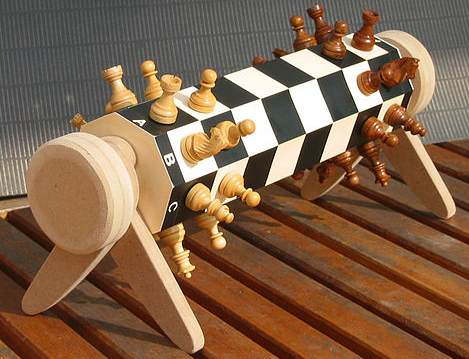
\includegraphics[width=0.75\textwidth]{Pictures/CoverPic.png}
    \caption{Vertical cylindrical chessboard with all pieces [4]}
    \label{fig:enter-label}
\end{figure}

\newpage
\begin{center}
\section*{1. Rules of the Game}
\end{center}

\indent In this paper we consider ordinary chess but played on different boards. In ordinary chess, we identify the files (columns) as letters a, b, ...h, and the rows from bottom to top as 1,2,...,8. In particular we consider cylindrical 8x8 chess. This is a board constructed from a standard 8x8 board by connecting the a file with the h file. Thus, for instance a white pawn on h4 can capture a black pawn on a5, and a knight on b2 can move to h3. Note that a knight on h1 can additionally move to a1 and a2, so that a checkmate in ordinary chess might not be a checkmate on a cylindrical board.

\vspace{0.5em}

\indent For most of this paper, we consider only king and pawn positions. As usual, kings move as in standard chess: one square in any direction with only horizontal wraparound allowed. Capture occurs diagonally forward, including across the edge (a pawn on a4 can capture a piece on h5). All pawns are equally connected due to the wraparound, and there are thus no edge pawns.

\vspace{0.5em}

\indent A pawn that reaches the 8th rank (White) or 1st rank (Black) is promoted and is treated as an immediate win. In fact, we usually treat any passed pawn as an immediate win.

\vspace{0.5em}

\indent En passant is allowed, including across the wraparound.

\vspace{0.5em}

\indent In pawn only positions (no kings), we count as a loss any player who has no moves. This can be converted to a standard chess position via the addition of a zugzwang (See 5. The Trebuchet Position for details).

\vspace{0.5em}

\indent There are no null moves: you must play on your turn

\vspace{0.5em}

\indent Standard win: checkmate the opponents king. Normal Play CGT (combinatorial game theory) win: a passed pawn for one player or a position where the opponent has no moves. We shall see later how to translate between a normal play win and a standard chess win via Trebuchet
positions.


\newpage
\indent We will first establish the basic positions of 0, 1, 2, $ \star $, $ \uparrow $, $ \downarrow $, and Tiny 1 using pawns (These are basic combinatorial games, see below). A very extensive discussion of these simple games 0, $\star$, 1, 2,.. $\uparrow$, ... can be found in [2]. In general we write $\{ a, b, \ldots \mid x, y, z, \ldots \}$ if white (left) can move to positions a,b,c... and black (right) can move to positions x,y,z......Next, we will add kings onto the board to treat bigger games as sum of smaller games under play. The main idea in these games comes from the trebuchet, which states that the first player to move loses. We will treat this as a zero game, making it easier to compute. We will then end our paper with the theories we developed to solve some chess puzzles. The format of this paper is heavily inspired by \textit{A Combinatorial Game Theoretic Analysis of Chess Endgames}[1] Note: we will be using standard 8 by 8 square chess boards in our diagrams, but we still consider the a-file and the h-file to be connected. Most of these analyses are essentially contained in [3], since they are equivalent to positions on an ordinary board.
\begin{center}
\section*{2. The Zero Game}
\end{center}
\indent  \indent Before we start looking at specific chess positions, let’s begin by defining the zero game: a game in which neither player can make a move. In combinatorial game theory (CGT) the notation is 0 = $\{|\}$. Under normal play, the zero game is a win for the second player. 

\begin{figure}[h]
    \centering
    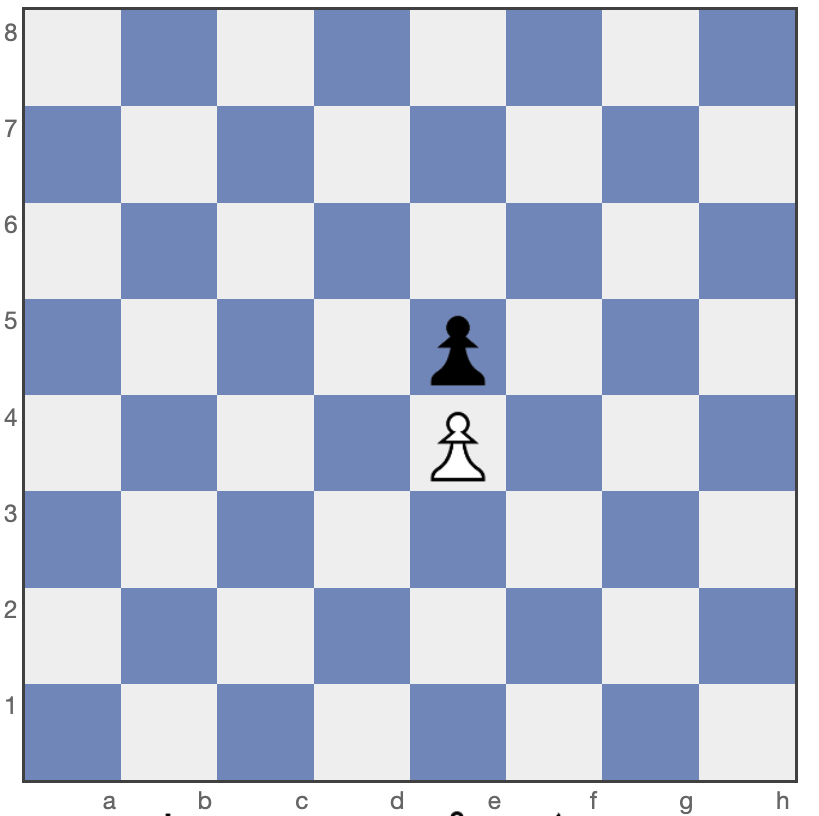
\includegraphics[width=0.5\textwidth]{Pictures/ZeroGame1.png}
    \caption*{Position 2.1 (position 2.1 [1]), (a-file and h-file are connected)}
    \label{fig:enter-label}
\end{figure}

\indent These two pawns in the center of the board are stuck, thus each side has no more moves. Hence,,this game is a second player win, meaning it's a zero game.

\newpage
\begin{figure}[h]
    \centering
    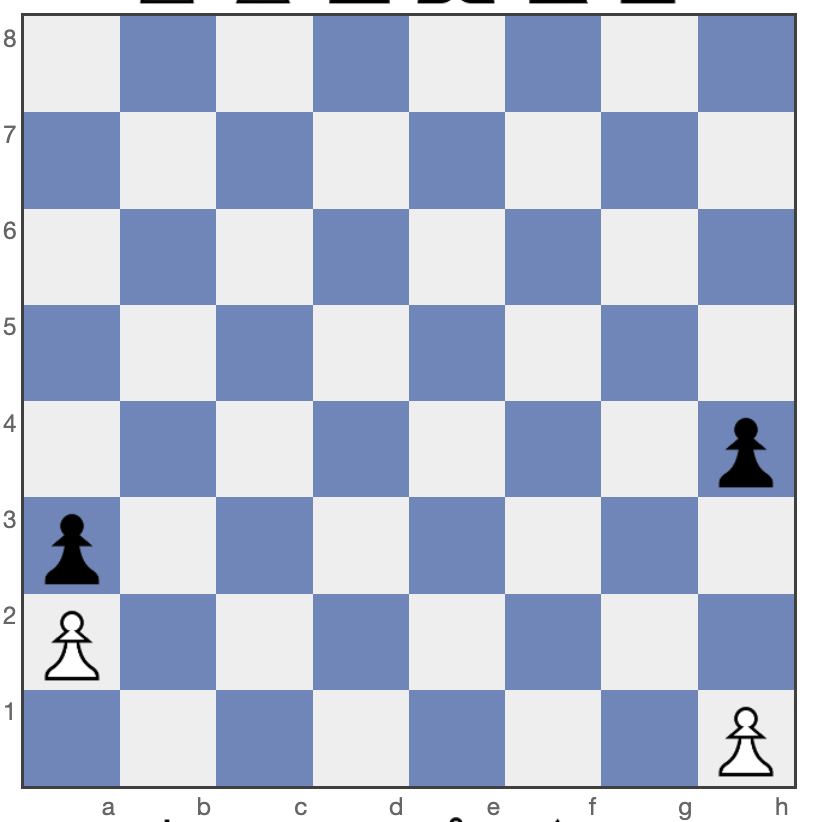
\includegraphics[width=0.5\textwidth]{Pictures/ZeroGame2.png}
    \caption*{Position 2.2, (a-file and h-file are connected)}
    \label{fig:enter-label}
\end{figure}

\indent In this position, if white goes first, it must move the h-file pawn, and the black pawn on the a-file will capture it, leading to a passed pawn and vice versa. This game is a second player win meaning this is a zero game. As said in [1] many of these zero games have symmetry across the board.
\vspace{0.5em}

\indent On a circular board, all files are equivalent, so that we could alternatively do the analysis with the pawns on the c and d files. Here is the "converted" board from cylindrical chess to ordinary. This is only possible when not all files are used and no checkmates via corner traps are used. 
\begin{figure}[h]
    \centering
    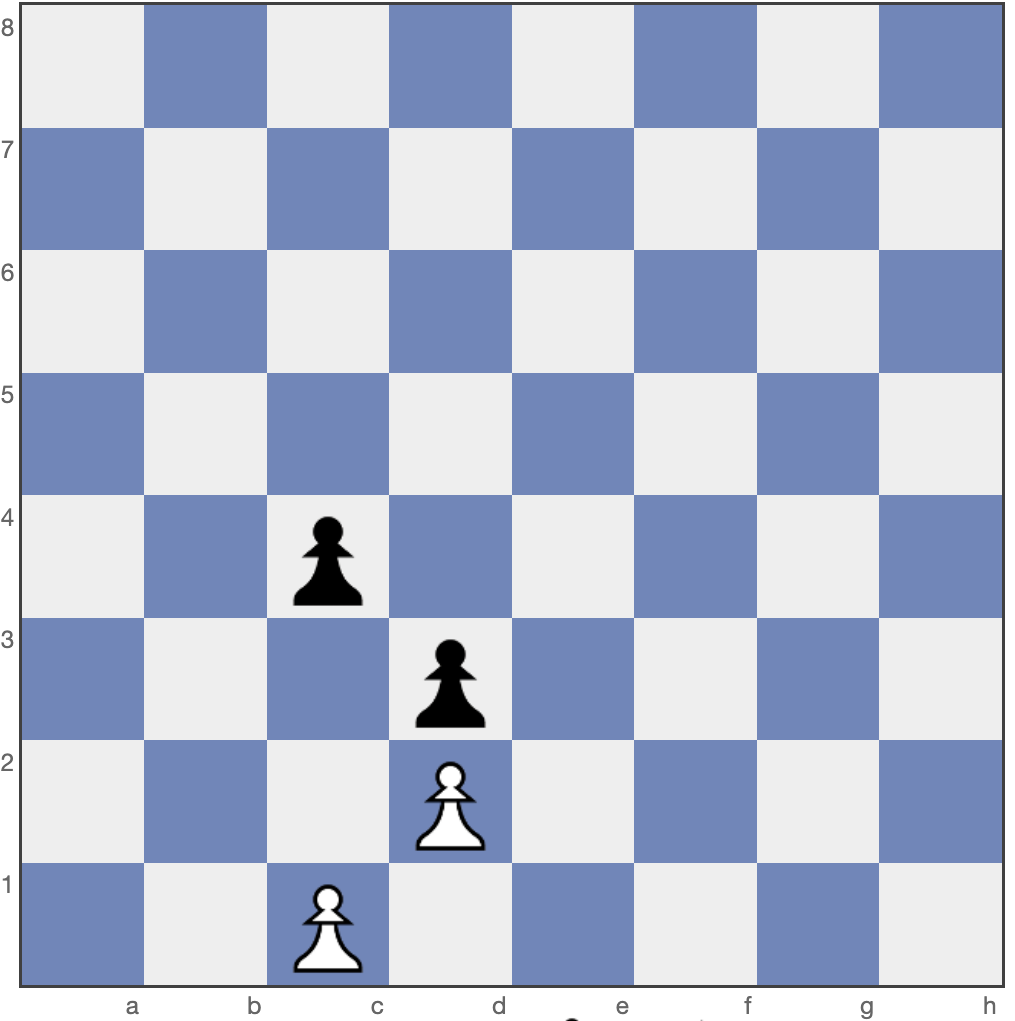
\includegraphics[width=0.5\textwidth]{Pictures/ZeroGame3.png}
    \caption*{Position 2.3 (position 2.1 [1])}
    \label{fig:enter-label}
\end{figure}

\begin{center}
\section*{3. The $\pm 1$ and $\pm 2$ Game}
\end{center}
\begin{figure}[h]
    \centering
    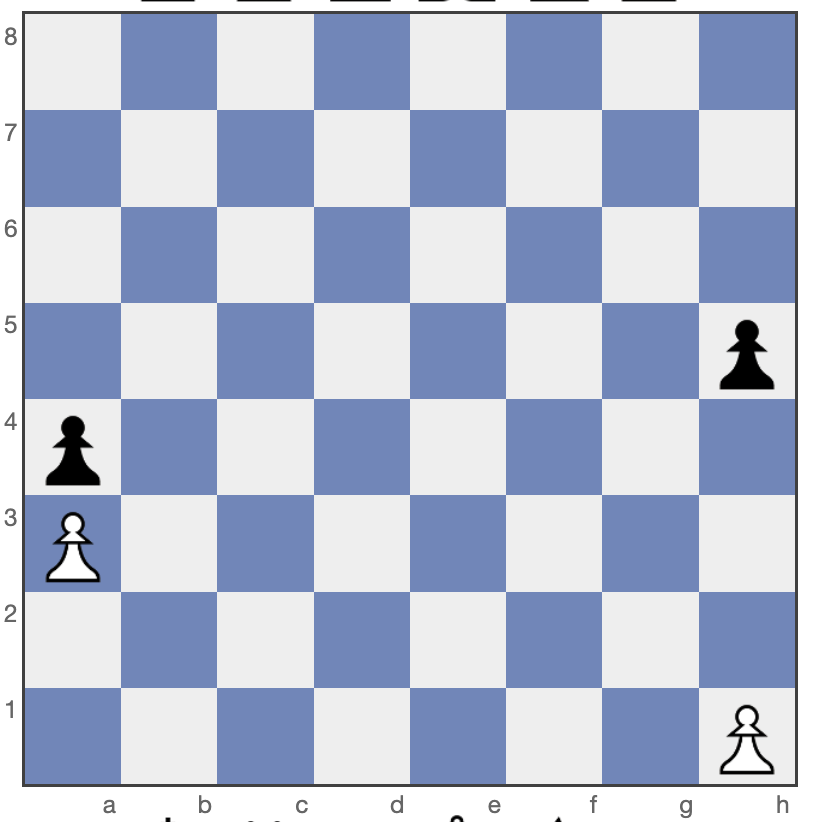
\includegraphics[width=0.5\textwidth]{Pictures/OneGame1.png}
    \caption*{Position 3.1, (a-file and h-file are connected)}
    \label{fig:enter-label}
\end{figure}
\[\]
\indent In this position the two deadlocked pawns remain the same, but the white pawn on the h file is moved back an extra square. In this game, white (left) can move to the zero, (position 2.2) and black (right) has only one move, which leads to a passed pawn by white. Thus, this game can be represented by G = $\{0 || \}$ which is defined as the one game. For this game to make complete sense, we will say that having all losing games is the same as having no moves at all [1]. 

\begin{figure}[h]
    \centering
    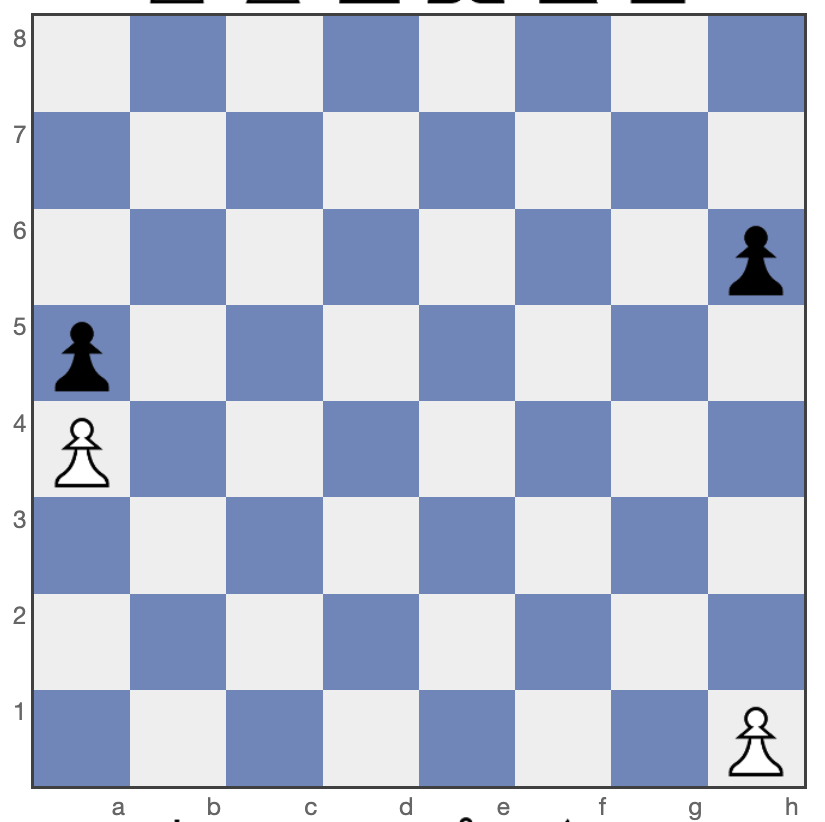
\includegraphics[width=0.5\textwidth]{Pictures/TwoGame1.png}
    \caption*{Position 3.2, (a-file and h-file are connected)}
    \label{fig:enter-label}
\end{figure}

\indent In this position, the two stalemated pawns remain the same, but the white pawn on the h file is moved back an extra square. In this game, white (left) can move to the zero game (position 2.2) or one game, (position 3.1) and black (right) has only losing moves. Thus, this game can be represented by G = $\{0, 1 || \}$ which is defined as the two game. 

\indent If one wanted to find the -1 or -2 game, all one would need to do is switch the black and white pieces and rotate the board 180 degrees [1]. 

\begin{center}
\section*{4. The Infinitesimals ($ \star $, $ \uparrow $, $ \downarrow $, Tiny 1) Games}
\end{center}

\begin{figure}[h]
    \centering
    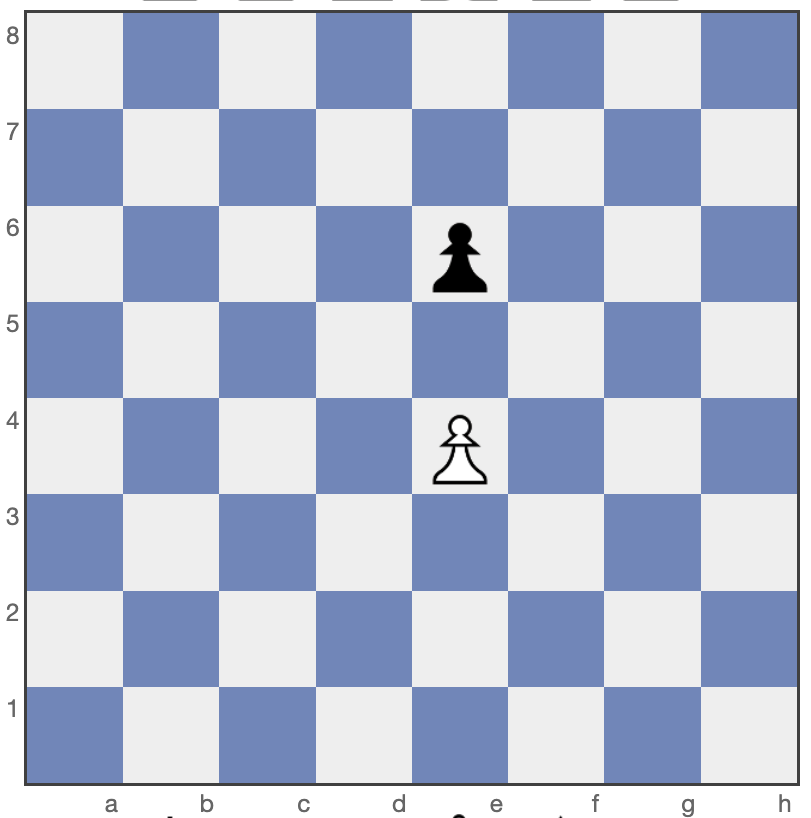
\includegraphics[width=0.5\textwidth]{Pictures/StarGame1.png}
    \caption*{Position 4.1 ([1] Position 4.1), (a-file and h-file are connected)}
    \label{fig:enter-label}
\end{figure}
\[\]
\indent The first position we will look at is $ \star $, which is when both white (left) and black(right) can move to the zero game. The formal definition of star is $ \star $ = $\{0 || 0\}$

\newpage
\begin{figure}[h]
    \centering
    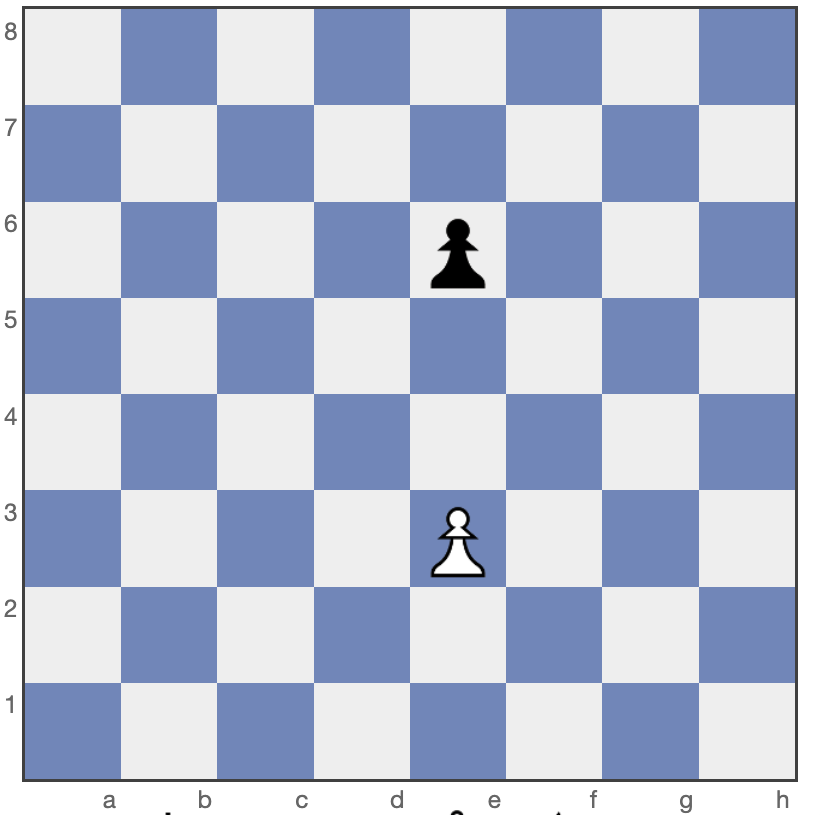
\includegraphics[width=0.5\textwidth]{Pictures/UpGame1.png}
    \caption*{Position 4.2 ([1] Position 4.2), (a-file and h-file are connected)}
    \label{fig:enter-label}
\end{figure}

\indent The formal definition of up is $\uparrow  = \{0 \mid *\}$. White(left)  can move to star or zero and black(right) can only move to star, thus $ G  = \{0, *\mid *\}$. $*$ is a reversible move for white(left) because the original game is greater than zero, and white will lose playing star as black will play zero and win [1]. Thus $ G  = \{0\mid *\} = \uparrow$. If we want to get $\downarrow$ we will do the same thing mentioned earlier by going from the 1 game to the -1 game.  

\begin{figure}[h]
    \centering
    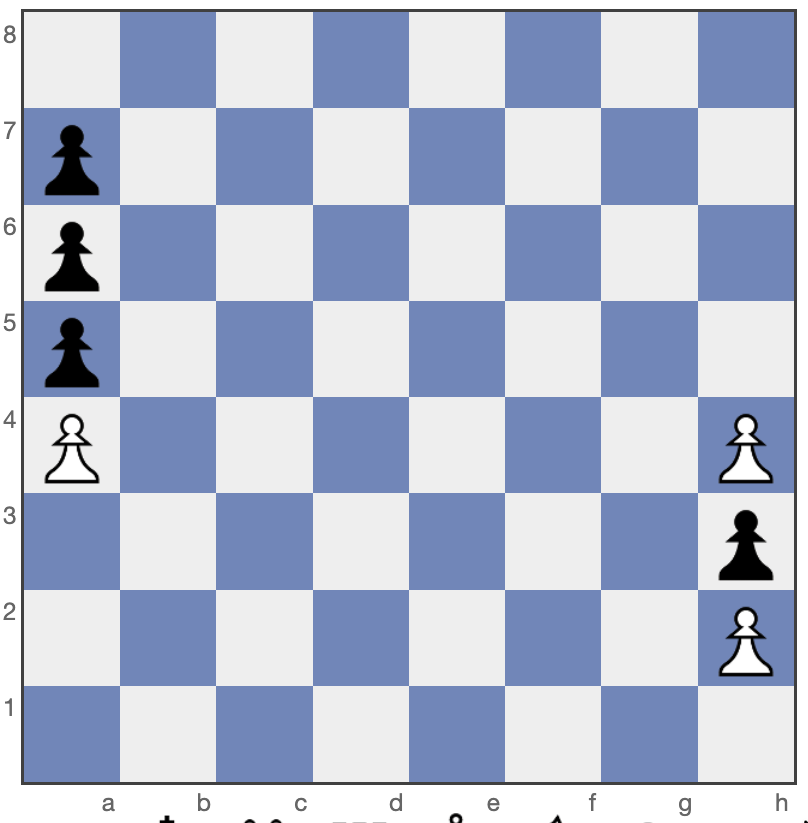
\includegraphics[width=0.5\textwidth]{Pictures/TinyGame1.png}
    \caption*{Position 4.3, (a-file and h-file are connected)}
    \label{fig:enter-label}
\end{figure}
\[\]
\indent Tiny 1 is defined as $\left\{ 0 \mid \left\{ 0 \mid -1 \right\} \right\}$. In this position, white can take the black pawn leading to a dead end, or white can advance leading, to a passed pawn for black. Black can only take white's pawn, which leaves us with the position $\left\{ 0 \| -1 \right\}$, giving us our desired answer. 

\begin{center}
\section*{5. The Trebuchet Position}
\end{center}
\begin{figure}[h]
    \centering
    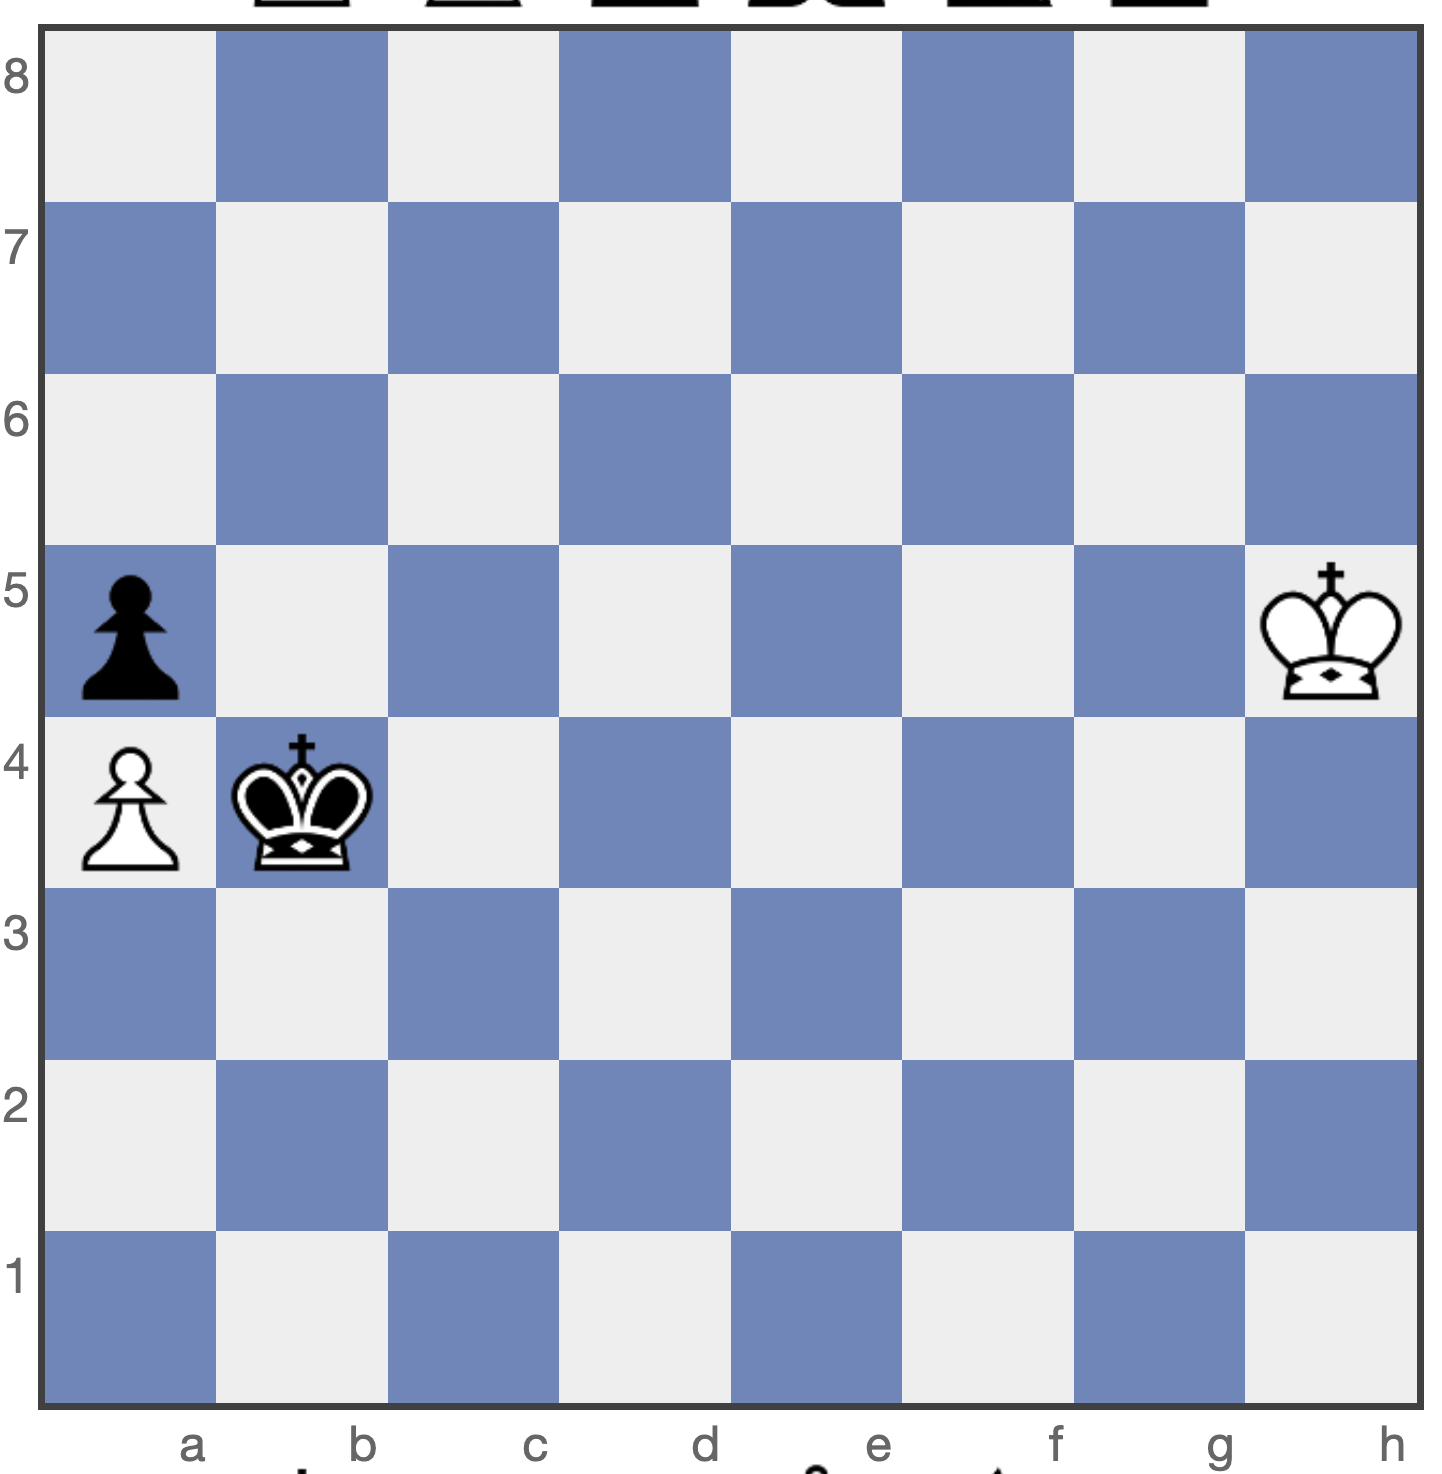
\includegraphics[width=0.5\textwidth]{Pictures/TrebuchetPosition1.png}
    \caption*{Position 5.1, (a-file and h-file are connected)}
    \label{fig:enter-label}
\end{figure}

\indent In this position, we introduce the king and have an example of mutual zugzwang in which the second player wins. Whichever player goes first will lose a pawn, allowing the other side's pawn to advance and promote. Thus this position is a zero game. This will be our default position for the kings for our upcoming chess puzzles. 

\begin{center}
\section*{6. Chess Strategies}
\end{center}

\indent Principle 1: The number avoidance theorem says that in a game which is the sum of numbers and not numbers, if one player can win, they can do so by not moving in the numbers. For the player, this indicates that they should not move in chess endgames that have a sum of games to not move in the numbers.[2, Pages 147-149]

\indent Principle 2: For any move, one should move to the game with the highest temperature. The temperature of an infinitesimal is 0, and the temperature of a switch game (a position where a player can choose between two or more distinct outcomes,) is $\{ x \parallel y \},\, x > y,\, \text{is}~\frac{(x-y)}{2}.$. This is not universally true, but will be true in all our examples.[2, Chapter 6]

\begin{center}
\item \section*{7. Chess Puzzles} 
\end{center}
\indent We will be studying 3 puzzles using what we have discussed thus far. 

\begin{figure}[h]
    \centering
    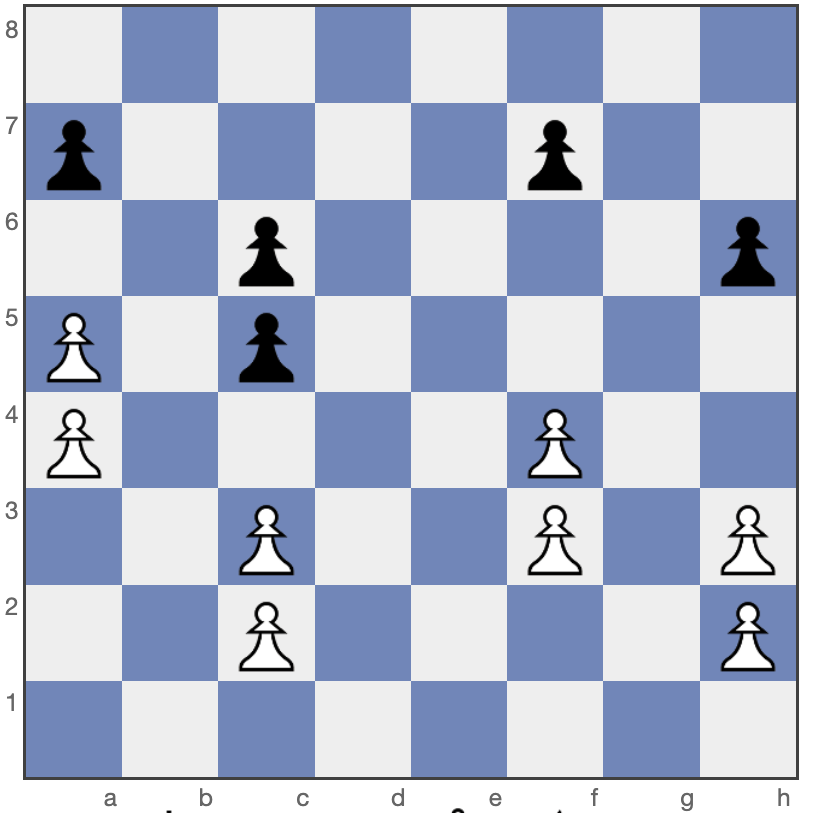
\includegraphics[width=0.5\textwidth]{Pictures/ChessPuzzle1.png}
    \caption*{Position 7.1, (a-file and h-file are connected), Diagram 8 [3]}
    \label{fig:enter-label}
\end{figure}

\indent The first thing to keep in mind is that we will break this position into multiple, smaller games. The first game is in the c-file, the second is in the f-file, and the last game is in the h and a-files. Let's first start with the c-file game, in which we have two pawns for white and black separated by one square. Thus, the first player to move wins, and $G = \left\{ 1 \mid -1 \right\} = \pm 1$. The next game we will start with is the f-file game, if white goes first it can move to f5. Black will move to f6 and white will move to f4, making it a win for white. If black goes first, it can either move to f5, resulting in black winning, or it can move to f6, leading to a white win. Thus, our game is $G = \left\{\,\left\{2\,\middle|\,1\right\}\,\middle|\,0\right\}$. Now let's focus on our last game, the a-file and h-file connected game. In this position, white wins all possible games. The best move for white (assuming white goes first) is to move the a-file pawn to a6, blocking black's pawn on the a-file; black is forced to move to h5, allowing white's pawn to capture. This leaves black to only capture white's piece, allowing white to promote and win. The best move for black, assuming black goes first, is to capture the a-file pawn and thus block white's second pawn on the a-file. This forces white's pawn on the h-file to advance, letting black capture white's pawn on the h-file. This leads to a zero game where black is the first to run out of any playable moves. Thus, this game is the one game, as white wins all possible moves. Thus, our final sum of this game is $\bm{G = 1 \pm 1 + \left\{\,\left\{2\,\middle|\,1\right\}\,\middle|\,0\right\}}$. 
\[\]
\begin{figure}[h]
    \centering
    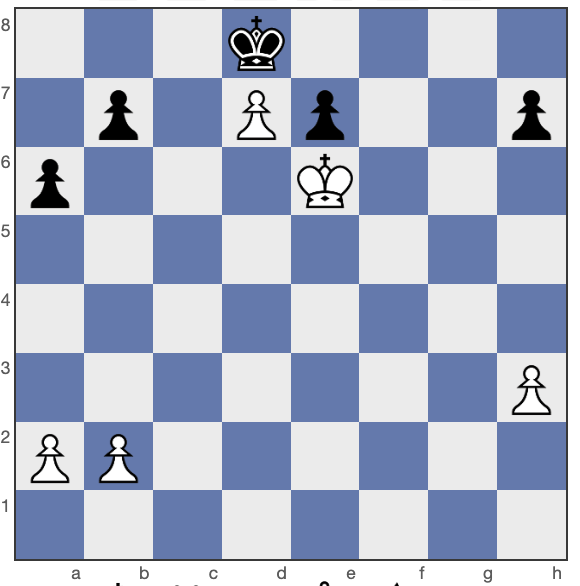
\includegraphics[width=0.5\textwidth]{Pictures/ChessPuzzle2.png}
    \caption*{Position 7.2, (a-file and h-file are connected)}
    \label{fig:enter-label}
\end{figure}
\[\]
\indent Similar to the last game, we will be breaking this bigger game into the sum of sums of smaller games. In this puzzle, we have finally added kings to make it a proper game, although it is in the Trebuchet position. The first game is the Trebuchet position, and the second game is the big game within the a,b, and h files as they are all connected. The first game, as we discussed earlier, is the zero game. Now let's move on to the next game with white starting first. White's best move is h4, and black counters with b5, as black's other two pawns prevent further white advancement. White's next move is a3, this is a brilliant move as it makes white's position symmetric to black's while being the second player. Black moves to h6, and white copies this move by moving to b3. Black's next move is h5, and white again copies playing b4. Black must play b5, allowing either pawn at b4 or h4 to take, leading to a passed pawn for white, and thus a win for white. Now, lets consider black going first. Black's first move is a5 which blocks white from moving to h4 and b4, and white moves to b3. Black's next move is b5 and white moves to a3. Black's brilliant move is h5, making black's position symmetric and making black the second player. If white advances either pawn at b4 or h4, black will win by making the last move; If white moves the pawn in the b-file then black wins via passed pawn. It is highly recommended that the reader try this puzzle on their own, as there are cases of symmetry that are not included in this analysis. In the second game the first player to move wins, thus this game is equal to $\pm 1$. Thus, our whole game is $\bm{G = 0 \pm 1}$.
\[\]
\begin{figure}[h]
    \centering
    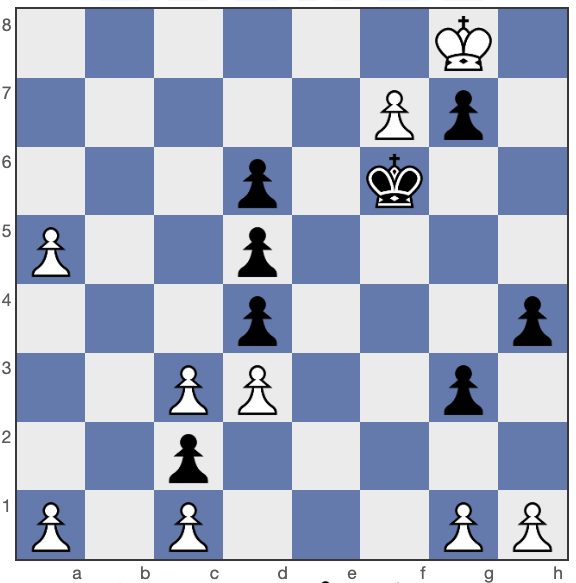
\includegraphics[width=0.5\textwidth]{Pictures/ChessPuzzle3.png}
    \caption*{Position 7.3, (a-file and h-file are connected)}
    \label{fig:enter-label}
\end{figure}
\[\]
\[\]

\indent This position was inspired by Diagram 9 [3]. In our board, we had to remove the knights as they would force us to block them using the other side's pawns and becomes more difficult with extra pawns being added to the game, creating more mini games. Thus, we have replaced the knights with pawns from the same side.  
\vspace{0.5em}

\indent Like the last two games, our approach to solving this game will be by breaking it down into smaller games. The first game is the Trebuchet position, the second game is in the c and d files, and the last game is g,h, and a file game. The first game, as we discussed earlier, is the zero game. For our second game we should note that white's pawn on c1 and black's pawn on c2 can't move, as they are both deadlocked and thus can't contribute to the game. If white goes first, it will take the black pawn on d4, leading to black having no moves left and making it a white win. If black goes first, its only playable move is black's pawn takes white's pawn on c3. This allows white to move to d4, leaving black with no playable moves. So our second game $G = 1$, as white wins in both cases. Now, lets move on to our last game. In this game, white's best move is just to promote its pawn on a5 and win the game. If white goes first, it moves its pawn to a6. Next black will move to g3 as its other pawn is blocked by white's pawn on h1. White will next move its pawn to h7, and black can play either g2 or h2. White will then move to h8, leading to promotion, thus this is a win for white. If black goes first, it will move its pawn to h3 and white will advance its pawn to a6. Now black can either move its pawn to g2 or h2; this will lead to a trading of black's pawns and white's pawns by capture but will either leave black with no playable moves or no black pieces. This leads to a white win again. Thus, the value of this third game is $G=1$. Our final game is $G = 0+1+1 = 2$. 

\begin{center}
\item \section*{8. Dawson's Chess and Its Ring Variant}
\end{center}

\indent Dawson's Chess is a combinatorial game played on a 1×n strip (or equivalently, a single row of n squares). Each square is initially occupied by a pawn. On each turn, a player must remove a pawn, but only if both its immediate neighbors (if any) are empty. The game ends when no moves are possible, and the last player to move wins. 
\vspace{0.5em}

\indent Dawson's Chess is an impartial game and can be analyzed using the Sprague-Grundy Theorem. The key result is that every position in Dawson's Chess is equivalent to a Nim heap of a certain size, called its Grundy number. The Grundy number for a row of length n is G(n). The formula from [2] $G(n) = \operatorname{mex} \left\{ G(a) \oplus G(b) \mid a + b = n - 3,\ a, b \geq 0 \right\}$, $\oplus$ being the bitwise XOR and mex being minimal excludant (the smallest non-negative integer not in the set). For the proof and reasoning behind this see [2]. 
\vspace{0.5em}

\indent Ring Dawson's Chess is a variant where the board is circular: the first and last squares are considered adjacent. This introduces a new position not present in the original version. The definition of this variant is the board consists of n pawns arranged in a circle. On each move, a player must remove a pawn, provided both its neighbors (now including the wrap-around) are empty, and the game ends when no moves are possible. 
\vspace{0.5em}

\indent In Ring Dawson's Chess, the only possible move from the full ring is to remove three consecutive pawns, leaving a segment of length $n-3$. Because the board is circular, all files (positions) are equivalent, and the resulting position is a linear Dawson's Chess of length $n-3$. Thus, the Grundy number for the ring is determined by the Grundy number of the linear game of size $n-3$: $\operatorname{Ring}(n) = \operatorname{mex}\left( G(n-3) \right)$. This means that if $G(n-3) = 0$, then $\operatorname{Ring}(n)=1$. if $G(n-3) \neq 0$, then $\operatorname{Ring}(n)=0$. So, the Grundy value for the ring is always either 0 or 1. 
\vspace{0.5em}

\indent The periodicity of Grundy numbers for regular Dawson's Chess [2] carries over to the ring variant. Since the Grundy number for the ring depends directly on $G(n-3)$, and since $G(n)$ is ultimately periodic, so is $\operatorname{Ring}(n)$.

\newpage
\begin{center}
\section*{Citations}
\end{center}

\par
\textbf{[1]} Wu, Q., Yü, F., \& Landry, M. (2020). A combinatorial game theoretic analysis of chess endgames. Unpublished manuscript. Retrieved June 2025, from \url{https://academic.timwylie.com/19CSCI4341F/{chess_endgames_wqy.pdf}
\par
\textbf{[2]} Berlekamp, E. R., Conway, J. H.,\& Guy, R. K. (1982). Winning Ways for Your Mathematical Plays (2nd ed., Vol. 1). Natick, MA: A K Peters.
\par
\textbf{[3]} Elkies, N. D. (1999). On numbers and endgames: Combinatorial game theory in chess endgames. In R. J. Nowakowski (Ed.), Games of No Chance (MSRI Publications No. 29, pp. 135--150). Cambridge: Cambridge University Press. Also available at arXiv:math/9905198 [math.CO].
\par
\textbf{[4]} Echecs Cylindriques Serge Clair [Image]. (n.d.). Wikimedia Commons. Retrieved June 2025, from \url{https://commons.wikimedia.org/wiki/File:EchecsCylindriquesSergeClair.jpg}
\par

\end{document}